\chapter{Methodology}
\index{Methodology@\emph{Methodology}}%
\label{chap:methodology}

\section{Overview}\label{sec:method overview}

To examine the effects of cooperativity-conscious schedulers we needed to have 
a method for comparing several scheduler implementations without needing to 
modify the underlying implementation of processes, channels, or application
source code. It would be also beneficial if our solution were able to visualize
these differences similar to Haskell's ThreadScope \cite{jones2009parallel}.

Our solution, $ErLam$, is a compiler for an experimental version of Lambda 
Calculus with Swap Channels and a runtime system which allows for swappable 
scheduler mechanisms and an optional logging system which can be fed into a 
custom report generator.
We break up our solution description into three parts; 
Section~\ref{sec:erlam}
will discuss our language syntax and semantics. It will also demonstrate our
Runtime Scheduler API by breaking down the CML Interactivity scheduler. 
Section~\ref{sec:simulation and visualization} 
will go more into depth about
our testing environment which involves our logging system, the report generator,
and the set of example applications we used to represent different cooperativity
levels. 
Finally, Section~\ref{sec:cooperativity mechanics} will go over our
example schedulers we wrote which demonstrate cooperative-conscious behavior. 
These will be the schedulers we provide our results against.

\section{ErLam}\label{sec:erlam}

The ErLam toolkit is itself broken down into three parts, the language and its
semantics, the Runtime System, and the Scheduler API. We will first lay out the
language and its basic semantics, as the finer-details are reliant on the exact
selected scheduling solution as well as the chosen swap-channel implementation.
We will then examine the possible channel implementations and how they effect
the given semantics. Next, we will discuss the Scheduler API using an example
scheduler implementation. We conclude this chapter with a summary of each of the 
classic schedulers that are included in the ErLam toolkit.

\subsection{The ErLam Language}\label{sec:the erlam language}

The ErLam Language is based on Lambda Calculus, with first-class single 
variable functions, but deviates somewhat in that it provides other first-class 
entities. It deviates from Church representation to provide Integers, this is
purely for ease of use. It also provides a symmetric synchronous Channel type 
for interprocess communication. As a note, this language can also be classified 
as a Simply-Typed Lambda Calculus.

\begin{figure} %% THE ERLAM LANGUAGE BNF WITHOUT SYNTAX SUGAR %%
\centering
{\footnotesize
    %%
%% ErLam BNF Style Grammar.
%%
\begin{BVerbatim}[commandchars=\\\{\}]
<Expression> ::= <Variable> 
              |  <Integer>
              |  `\textbf{newchan}'
              |  `\textbf{(}' <Expression> `\textbf{)}'
              |  <Expression> <Expression>
              |  `\textbf{if}' <Expression> <Expression> <Expression>
              |  `\textbf{swap}' <Channel> <Expression>
              |  `\textbf{spawn}' <Expression>
              |  `\textbf{fun}' <Variable> `\textbf{.}' <Expression>
\end{BVerbatim}

}
\caption{The ErLam language grammar, without syntax sugar or types.}
\label{fig:grammer}
\end{figure}

Figure~\ref{fig:grammer} expresses ErLam in its simplified BN-Form. The 
semantics for the language is fairly straight forward, but its operational 
semantics are layed out in appendix~\ref{app:semantics}. All expressions reduce
to one of the terminal types: Integer, Channel, or Function. To spawn for 
instance, if any terminal is passed other than a function, it returns a $0$
(\eg~false). When a function is passed, it is applied with $nil$ to 
initialize the internal expression in another ErLam process, and evaluates to $1$ (\eg~true) in the parent process.

ErLam also makes a number of ease-of-use decisions like providing a default 
branch operator and a library system for providing a set of built in functions 
such as numeric operations, type checking, and standard functional behaviors 
(\eg~combinators, \etc). However, these built-ins will be largely ignored in 
this document but explained when neccessary. 

ErLam also extends this base grammar with some useful syntactic sugar (see 
figure~\ref{fig:sugar-transform} for syntactic transformations) such as SML 
style $let$ expressions and multi-variable function definitions (which are 
curried from left to right). We will use the syntactic sugar throughout this 
document to make our source easier to review.

\begin{figure}
    \centering
    \begin{align*}
        \textbf{let}\: x\: =\: e_1\: \textbf{in}\: e_2
        & \Rightarrow
        ((\textbf{fun}\: x.e_2)\; e_1) \\
% 
        \textbf{fun}\: \textit{x,y,z} . \textit{e}
        & \Rightarrow
        \textbf{fun}\: \textit{x} . (\textbf{fun}\: \textit{y} . (\textbf{fun}\: \textit{z} . \textit{e} ))
    \end{align*}
    \caption{Syntactic sugar parse transformations.}
    \label{fig:sugar-transform}
\end{figure}

Also, note the possible steps \emph{swap} can take: either returning a block
or another expression and a set of functions. On a semantic level,
either event is transparent and results in blocking behaviour until a successful swap.
However, in the former case, the channel has blocked and the only course of 
action for the scheduler is to get another expression to work on. In the 
later case, we have an expression to work on, but we also may have unblocked 
other processes by doing so, so we need to reschedule them. 
Note that in this case the function set may be null and the expression returned may be
another attempt at swapping (\ie~$e = (\textbf{swap}\:c\:v)$). This would let 
the scheduler choose whether to retry immediately or reschedule it for a later
time and work on something in the mean time. Thus, there are several possible
channel implementations we could provide while still adhering to the above
semantics.

\subsection{Channel Implementations}\label{sec:channel implementations}

ErLam provides a selection of channel implementations to allow for 
interchangeable scheduler comparisons with different synchronization methods.
We chose two channel implementations the 
{\sl Blocking} Swap, and the {\sl Absorbing} Swap as they highlight key differences
for the runtime. We will now look at an example application and its execution
using both methods for comparison.

\begin{wrapfigure}{r}{0.5\textwidth}
    \centering
{\footnotesize
\begin{BVerbatim}[commandchars=\\\{\}]
\textbf{let} c = \textbf{newchan in}
\textbf{let} f = (\textbf{fun} _.(\textbf{swap} c \textit{42})) \textbf{in}
\textbf{let} _ = (\textbf{spawn} f)
\textbf{in} (\textbf{swap} c \textit{0})
\end{BVerbatim}
}
    \caption{
        A simple ErLam application which swaps on a channel before returning.}
    \label{fig:swap-example}
\end{wrapfigure}

Figure~\ref{fig:swap-example} gives an example ErLam application. It first 
creates a new channel for processes to communicate on. It then creates a 
null-function to spawn, whose sole purpose is to swap on the channel the number
$42$ and quit. Finally, it swaps on the channel the number $0$ and returns
the result of the whole evaluation, which in this case will be the value passed
from the other end of the swap, $42$. 

As ErLam is innately concurrent, we do not know which process will ask to swap
first. It may even be possible that $0$ asks to swap several times before $42$
even tries. In fact, the {\sl Blocking} channel allows this behaviour of 
multiple swap attempts.
We can see an illustration of this in figure~\ref{fig:blockchan-example}.
The first row shows the arbitrary time-slice $t_1$ where the process swapping $0$, 
$p0$, first contacts the channel with its value. The process may be scheduled again,
repeatedly, to check the channel up to some arbitrary time-slice $t_{n-1}$. At
$t_n$ however, the process swapping $42$ requests a swap and immediately gets a
value back and logs that the process which it swapped with can get its value
when it returns. Thus on the third line, for any arbitrary time-slice in the 
future $t_{>n}$, the process $p0$ can ask for a swap and get the value $p1$ 
stored.

Note the illustration makes no explicit mention of the scheduler or its 
functionality. It may be the case that the two processes are on different 
processing units and are in different process queues. 
Or it may be the case that they both exist in the
same queue and upon a block, the scheduler chooses the next one, which will 
immediately unblock the channel.

\begin{figure}
    \makebox[\textwidth][c]{
\subfigure[t][Process Blocking Swap]{
    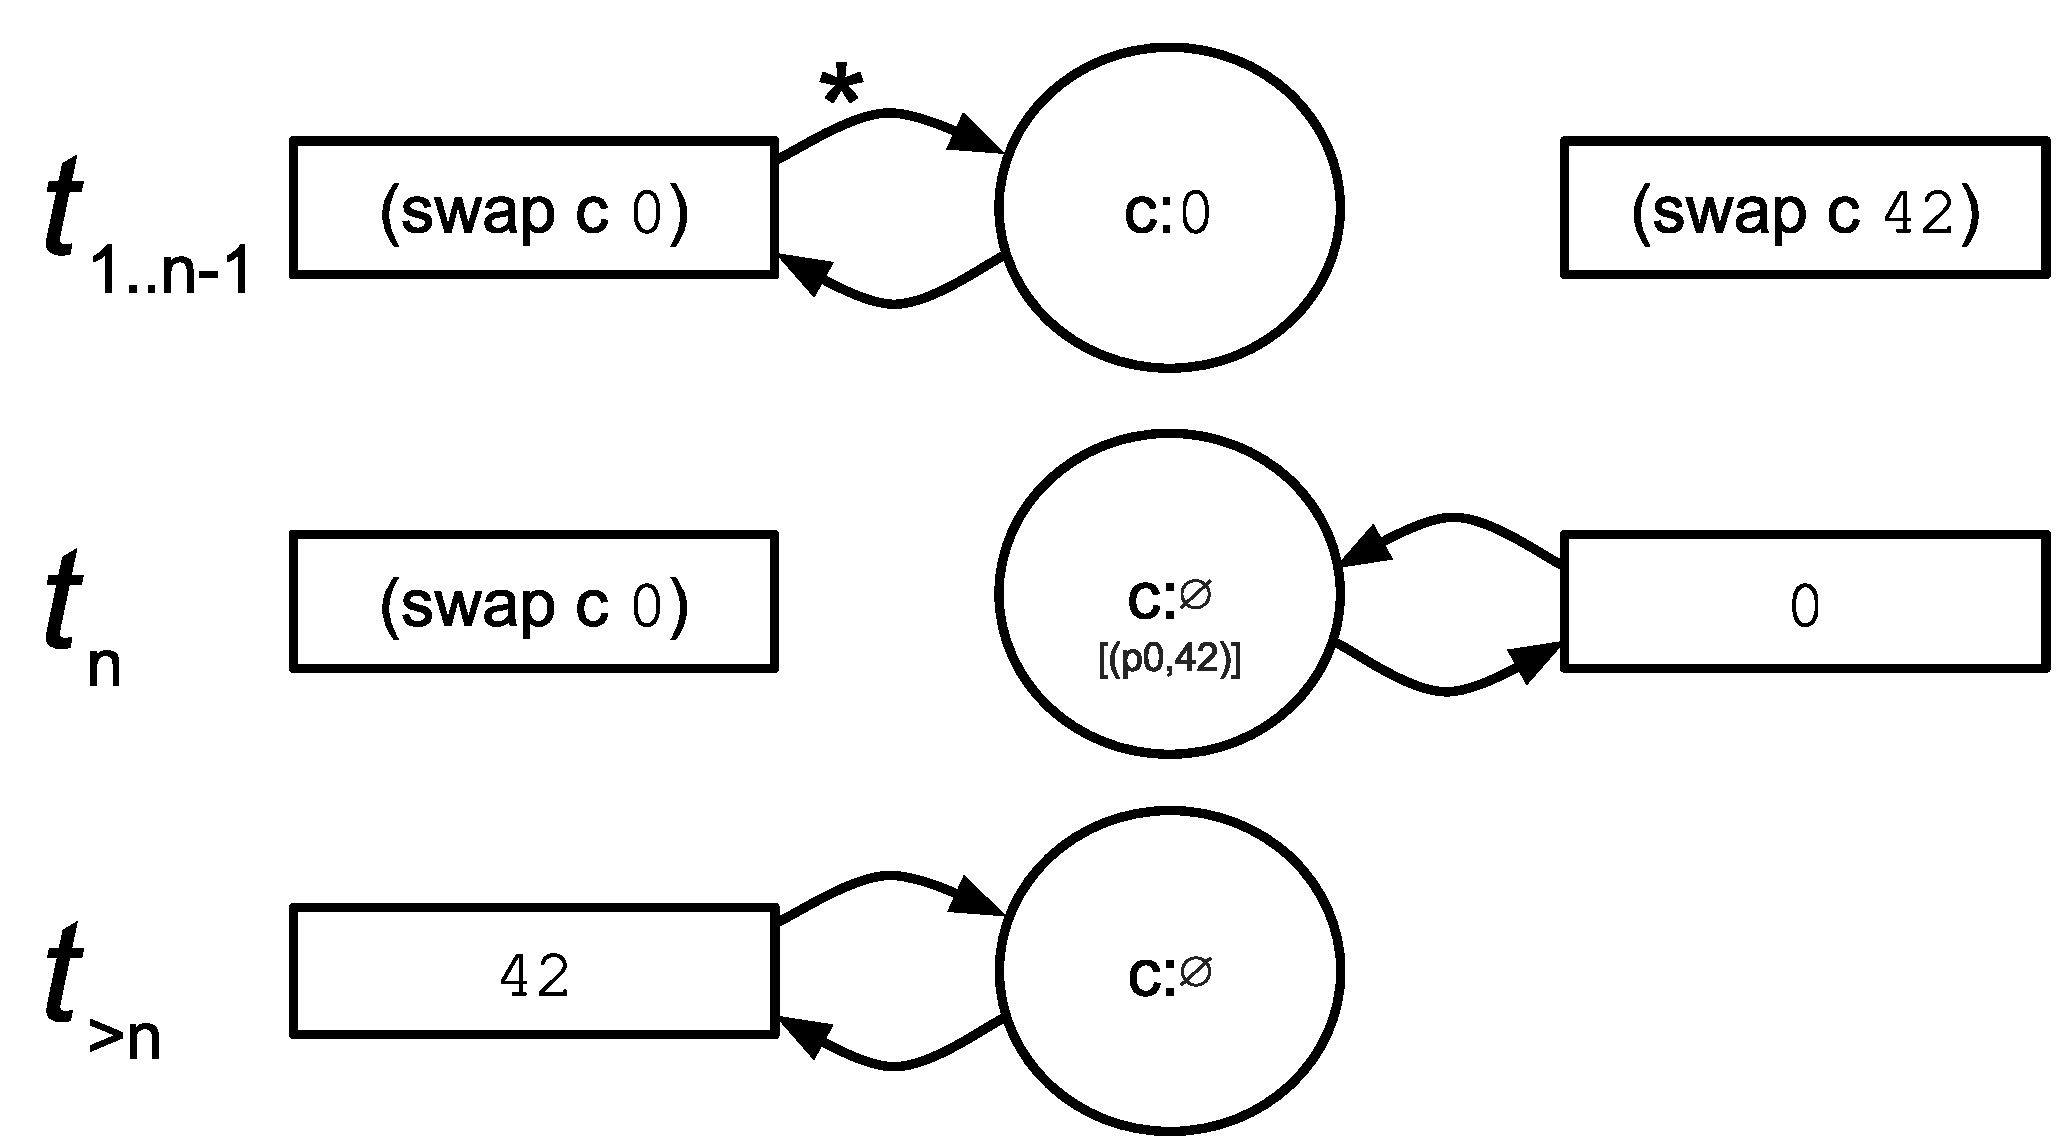
\includegraphics[scale=0.25]{BlockingSwap.pdf}
    \label{fig:blockchan-example}
}  \subfigure[t][Process Absorption Swap]{
    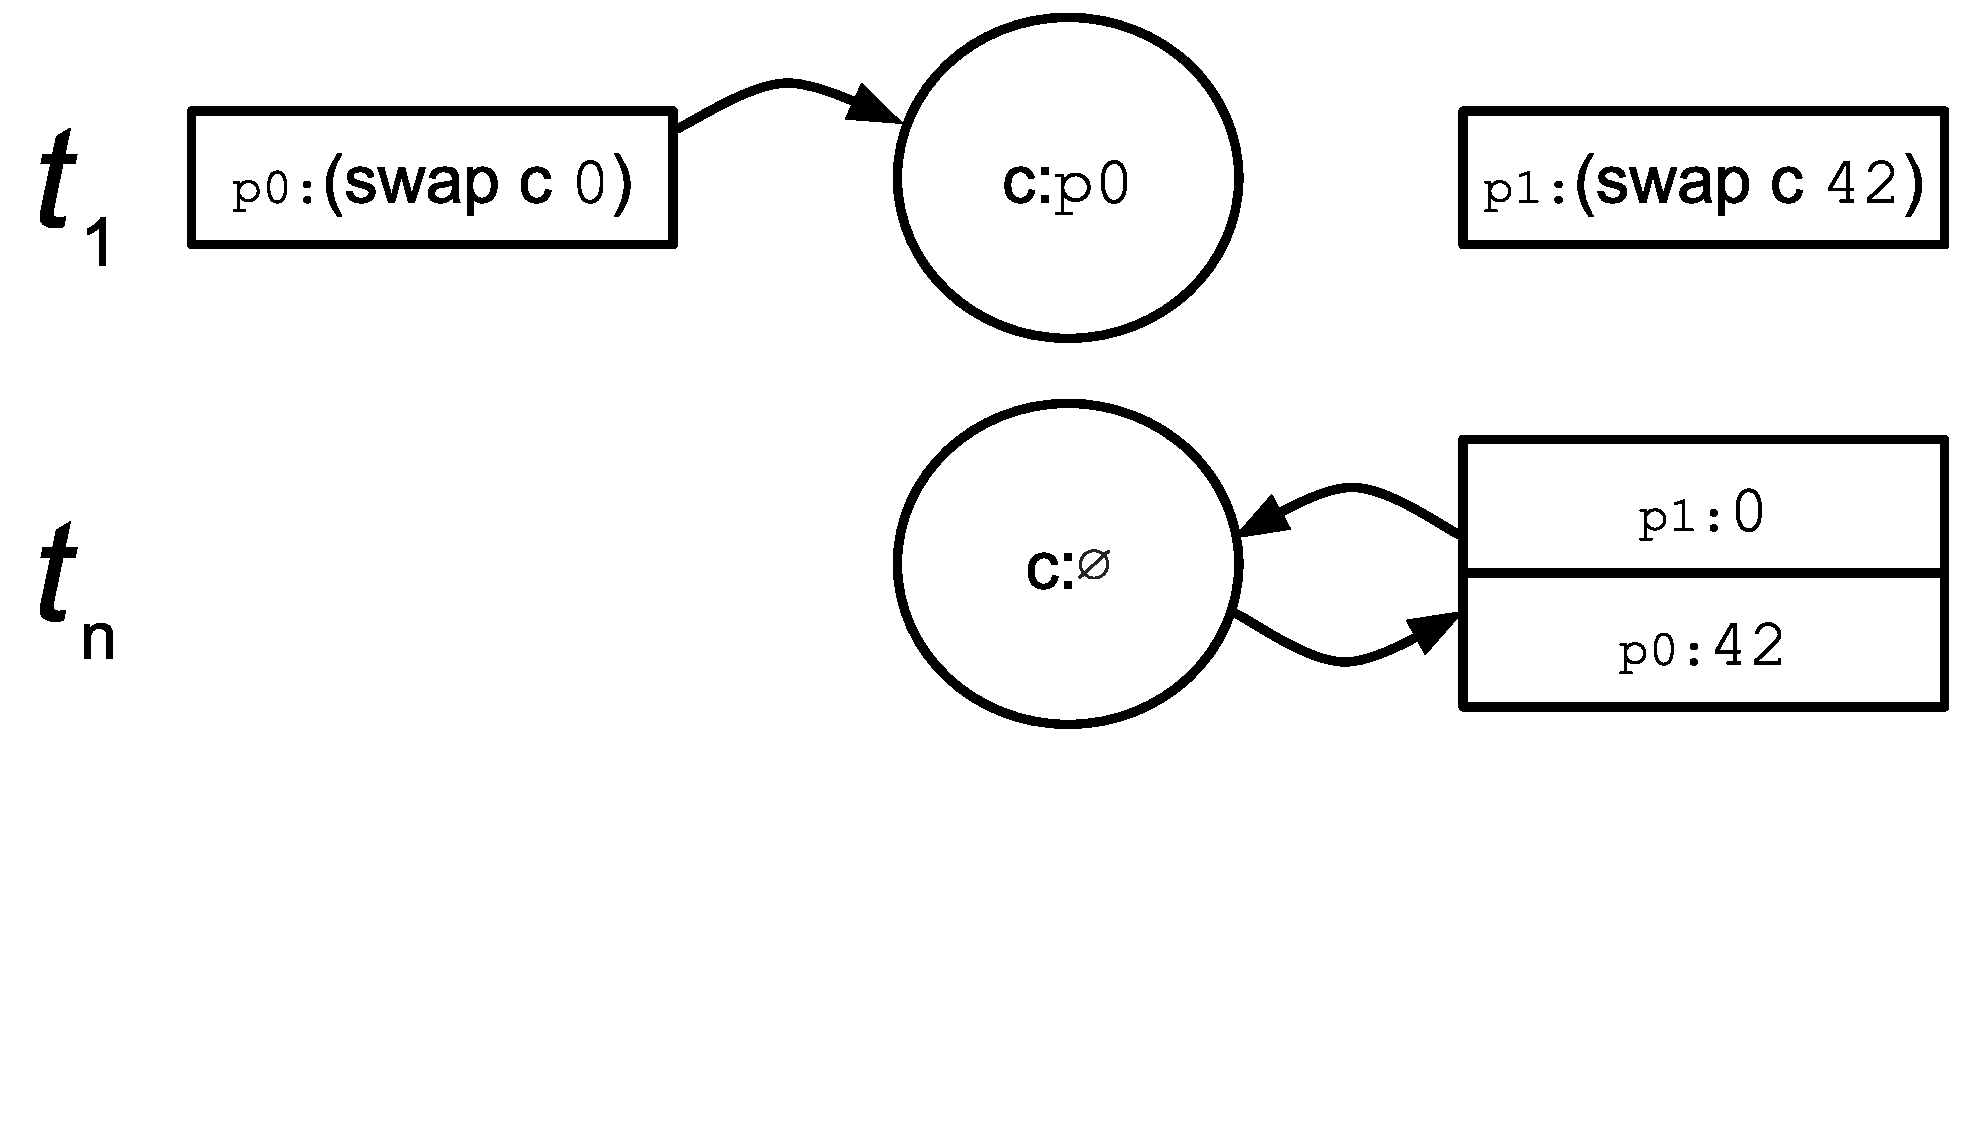
\includegraphics[scale=0.25]{AbsorbSwap2.pdf}
    \label{fig:absorbchan-example}
}}
\caption{Channel operation over time. Note arbitrary time-slice $t_1$ is when the 
first swap operation is evaluated.}
\end{figure}

The {\sl Blocking} channel effectively simulates a common spin-lock over a shared 
piece of memory. These channels represent a worst-case, albeit common, application 
implementation for concurrent software. Even so, they do allow for some hints
to the scheduler, which can be taken advantage of. Alternatives on the spin-lock 
could be added to the ErLam toolkit though, such as a push-notifying semaphore, 
however we provide a simpler and functionally more common alternative: the process 
absorption channel.

In the {\sl Absorption} channel (figure~\ref{fig:absorbchan-example}), the first 
process to get to the channel will get absorbed by it. The scheduler which 
evaluated the swap will be out a process, and but the scheduler which unblocks the channel 
by arriving second will get back two processes (the one performing the swap, 
and the absorbed one). In terms of scheduling efficiency this type of message
passing channel has provided enormous improvements for run-times which do not
wish to introduce channel inspection into their scheduler.

\subsection{The Scheduler API}\label{sec:the scheduler api}

ErLam was written in Erlang, and as such, can take advantage of Erlang's 
callback behaviour specifications. An \emph{erlam\_scheduler} behaviour was
defined which requires a minimum of $5$ callback functions 
(figure~\ref{fig:scheduler-api}).

\begin{figure}
    \begin{minted}[frame=lines,fontsize=\footnotesize]{erlang}
-callback layout( erlang:cpu_topology(), scheduler_opts() ) -> 
                scheduler_layout().

-callback init( scheduler_opts() ) -> 
                {ok, scheduler_state()} |
                {error, log_msg()}      |
                {warn, log_msg(), scheduler_state()}.

-callback cleanup( scheduler_state() ) -> 
                ok | {error, log_msg()} | {warn, log_msg()}.

-callback tick( scheduler_status(), scheduler_state() ) -> 
                {ok, scheduler_status(), scheduler_state()} |
                {return, term()} | {stop, scheduler_state()}. 

-callback spawn_process( erlam_process(), scheduler_state() ) -> 
                {ok, scheduler_state()} | {error, log_msg()}.
\end{minted}
\caption{The ErLam Scheduler API}
\label{fig:scheduler-api}
\end{figure}

Upon instantiation the runtime system will call the 
\emph{layout/2} function with the Non-uniform Memory Access (NUMA) layout 
of the system that the application is
running on, along with any parameters the user specified at runtime. The 
result of this function is to be the scheduler layout. 

For example, let's assume we are running our application on a Intel Core i7 
which has 4 logical cores which support hyper-threading. The \emph{layout/2}
function will be given the following structure: 

{\footnotesize 
\begin{verbatim}
   [{processor,[{core,[{thread,{logical,0}},{thread,{logical,1}}]},
                {core,[{thread,{logical,2}},{thread,{logical,3}}]},
                {core,[{thread,{logical,4}},{thread,{logical,5}}]},
                {core,[{thread,{logical,6}},{thread,{logical,7}}]}]}].
\end{verbatim}
} 

\noindent
This indicates to the scheduler implementation that it, at max, can spawn $8$
instances of itself which would be bound to each logical processing unit (LPU).
Although we could of course have a scheduler which acts differently based on the
architecture. However, the schedulers we have limited ourselves to are either
single or fully multi-core (\ie~uses all available LPUs).

To spin up an instance of the scheduler on the particular core, the 
\emph{init/1} function is called which should return the scheduler's state. 
As Erlang is a functional language, we use this state object as a means to
maintain some global state for each scheduler process by threading it through
all subsequent callback calls. Upon shutdown, the opposite function 
\emph{cleanup/1} is called.

The last two functions are the most interesting as they pertain to the core of
what each new scheduler provides, namely how to evaluate the world in a given
time-slice (\emph{tick/2}) and how a new process should be handled 
(\emph{spawn\_process/2}). An explanation of these callbacks is best done 
through example.

\subsection{Example Usage: The CML Scheduler}\label{sec:example the cml scheduler}

CML's scheduler utilizes a dual-queue structure rather than
a simple unary-process-queue. The scheduler attempts to differentiate between
{\em communication} and {\em computation}-bound processes so as to reduce the
effects of highly computationally intensive processes from choking the system.
The scheduling system thus improves on application interactivity by demoting 
{\em computation}-bound processes to the secondary queue (which isn't accessed
until another process is demoted).

Spawning a process in the CML scheduler (figure~\ref{fig:cml-spawn-process}) 
does not go onto the primary queue, instead we enqueue the current process and 
start evaluating the new process. This is a fairly simplistic example, but it 
shows how one would go about updating the state between ticks. Note also, that
the \emph{spawn\_process/2} call happens on the same scheduler instance which
evaluated the $spawn$. While this is not of consequence for this scheduler, a
multi-core scheduler could be confident in appending a new process to its local
queue without interfering with another LPU's scheduler.

\begin{figure}
\begin{minted}[frame=lines,fontsize=\footnotesize]{erlang}
spawn_process( Process, State ) -> 
    enqueueAndSwitchCurThread( Process, State ).

enqueueAndSwitchCurThread( Process, #state{curThread=T}=State ) ->
    case T of
        nil ->
            setCurThread( Process, State );
        _   ->
            % New process takes over
            {ok, NewState} = enqueue1( T, State ), 
            setCurThread( Process, NewState )
    end.
\end{minted}
\caption{CML Process Spawning.}
\label{fig:cml-spawn-process}
\end{figure}

In the original CML scheduler, it defined a quantum which it would let the 
current process run for, it would preempt it if it attempted to run 
for longer. The ErLam runtime avoids the use of time based quantum as logging 
and other factors directly effect the usefulness of this. Instead it uses a 
`tick', which emulates one
step forward in the execution of the application. Thus to simulate a quantum we
instead keep track of the number of reductions performed on the current process
and decrement the counter until we reach $0$.

\begin{figure}
\begin{minted}[frame=lines,fontsize=\footnotesize]{erlang}
tick( _Status, #state{ curReduct=0 }=State ) ->
    {ok, NState} =  pick_next( State ),
    reduce( NState );
tick( _Status, State ) -> reduce( State ).

pick_next( State ) ->
    {ok, NewState} = preempt( State ),      % Place cur thread onto queue
    {ok, Top, Next} = dequeue1( NewState ), % Pop next off
    setCurThread( Top, Next ).              % Set as cur and return state
\end{minted}
\caption{CML Process evaluation.}
\label{fig:cml-tick}
\end{figure}

The \emph{tick/2} function (figure~\ref{fig:cml-tick}) performs one of two 
things based on what the state of the system is. If the current reduction count 
is $0$, then we can pick a new process from the queue, otherwise we can perform
a reduction. 

Note for our scheduler simulation we ignore the first parameter to the 
\emph{tick/2} function for either case. The first parameter was the status of 
the scheduler returned from the previous tick (\eg~running, waiting, \etc). This 
would be useful if the CML scheduler utilized work-stealing to get work to do
from other LPUs when in \emph{waiting} mode.

\subsection{Provided Schedulers}

Along with the Single-Threaded Dual-Queue CML scheduler {\sl (STDQ)}, ErLam 
comes with several basic scheduling mechanics. We utilize these as bases cases 
on which to compare the behaviour of all subsequent feedback-enabled schedulers.

\begin{itemize}
    \item {\bf The Single-Threaded Round-Robin Scheduler {\sl (STRR)}} \\
        This scheduler uses a single FIFO queue which all processes are spawned 
        to. There is no rearrangement of order, and the single-thread scheduler 
        will just round-robin the queue performing a set number of reductions
        per process before enqueuing and poping the next one.

    \item {\bf The Multi-Threaded Round-Robin Global-Queue Scheduler {\sl (MTRRGQ)}} \\
        A multi-core version of the previous scheduler. This uses a single global
        process queue which all schedulers share and attempt to work from.

    \item {\bf The Multi-Threaded Round-Robin Work-Stealing Scheduler {\sl (MTRRWS)}} \\
        An improvement on the previous scheduler. Instead of a global process 
        queue, each scheduler maintains their own. A waiting scheduler will randomly 
        sleep-and-steal until it finds a process to work on from another scheduler. 
        The provided implementation gives two example stealing mechanisms:
        \begin{itemize}
            \item {\bf Shared-Queue {\sl (MTRRWS-SQ)}} \\
                Stealing a process involves performing an atomic dequeue from 
                the bottom (rather than the top) of another scheduler's process 
                queue. This will only block the other scheduler from performing
                a dequeue for a very short window of time, but involves 
                accessing "remote" memory.
            \item {\bf Interrupting-Steal {\sl (MTRRWS-IS)}} \\
                Simulates sending a thief-process over to another scheduler.
                When the victim scheduler preempts or yields their current process
                and selects the next one from the queue, they will instead get a
                thief process which will syphon a process away to spawn on the thief's home
                scheduler. This blocks the process for a longer period of time,
                but does not involve accessing remote memory.
        \end{itemize}
\end{itemize}

ErLam also comes with three cooperativity-conscious schedulers: the 
Longevity-Based Batching Scheduler (section~\ref{sec:longevity based batching}),
the Channel Pinning Scheduler (section~\ref{sec:channel pinning}), and the
Bipartite Graph Aided Sorting Scheduler (section~\ref{sec:bipartite graph aided sorting}).
The first two build on the same shared queue module as provided by $MTRRWS-^{*}$, 
while the third utilizes its own implementation.

For any compiled ErLam script, the runtime installs a command line option for
selecting the scheduler used (among several other options). We are able to 
specify that we wish to run $pfib$, for example, with $MTRRGQ$ with
the following command:
\begin{verbatim}
            ./pfib -s erlam_sched_global_queue 
\end{verbatim}
\noindent
Any new schedulers can be added to the ErLam toolkit without needing to 
recompile the scripts as they are dynamically fetched and loaded at runtime. 

\section{Simulation \& Visualization}\label{sec:simulation and visualization}

The second primary goal of the ErLam toolkit was the ability to visualize 
how a scheduler proceeded to evaluate an ErLam application. We therefore needed
a way to log all events over time, including unique per-scheduler events, such 
as the size of both the primary and secondary queues in the CML scheduler. It 
would also be advantageous to be as finely grained as possible and leave it up to 
the visualization mechanism to dial the accuracy.

We also needed a sample set of application simulations to run our set of 
schedulers against. These simulations needed to be minimal to reduce
extraneous data but still demonstrate various levels of cooperativity and phase 
changes. We would like to also have the ability to compose test cases 
together to better create realistic work-sets for the schedulers to react to.

\subsection{Runtime Log Reports}\label{sec:runtime log reports}

Logging in Erlang is a fairly simple matter. We utilize a simplistic data 
logging module based on syslog. The output of running an application 
could look like this:

{\footnotesize
\begin{verbatim}
                    timestamp,lpu,event,value
                    ...
                    983847.935268,3,sched_state,running
                    983847.935333,0,queue_length,59
                    983847.935677,24,channel_blocked,6102
                    983847.935683,6,yield,""
                    983847.936003,4,queue_length,50
                    983847.936430,3,tick,""
                    983847.936439,3,reduction,""
                    ...
\end{verbatim}
}
\noindent
The time-stamp given is a concatenation of the second and microsecond that the
event happened in. The lpu is the scheduler which caused the event, unless it's
a channel based event, such as a \emph{channel\_blocked} event, in which case it's
the channel ID. 

Our logging API is fairly simplistic as we only need to capture two types of metrics
from our events: quantity and frequency. With frequency, we want to know the
amount of events which happened in a time range, but with quantity we would like 
things like length of the scheduler's process queue over time or the amount of
time spent in the running or waiting state.

Note time is not consistent per LPU, it may be the case that another OS 
application is getting time instead of one of the ErLam schedulers. This could
result in one or more of the LPUs getting far less \emph{``tick''} events. Worse
yet, there may be a large gap of time missing from one scheduler to the next.
For our purposes though we would like to compare the state of the scheduler
while it is executing and would be fine with averaging over the largest gap. These
from experimentation have not been found to be very frequent or large on an
otherwise unoccupied processor (see section~\ref{sec:results-evaluation-classical} 
for details).

To explain this averaging technique we'll now discuss the report generation 
method. The ErLam toolkit comes with a secondary R script which can be given a 
generated log file for processing. This script dynamically loads chart 
creation scripts based on the types of events it sees in the log file. The
toolkit comes with five charting scripts which should work for all schedulers: 
Channel Usage (Communication Density) over time,
Channel State (blocked vs. unblocked) over time,
Process Queue Length per LPU over time,
Reductions (Computation Density) over time, and
Scheduler State (running vs waiting) over time.

%\begin{wrapfigure}{r}{0.5\textwidth}
\begin{figure}
\centering
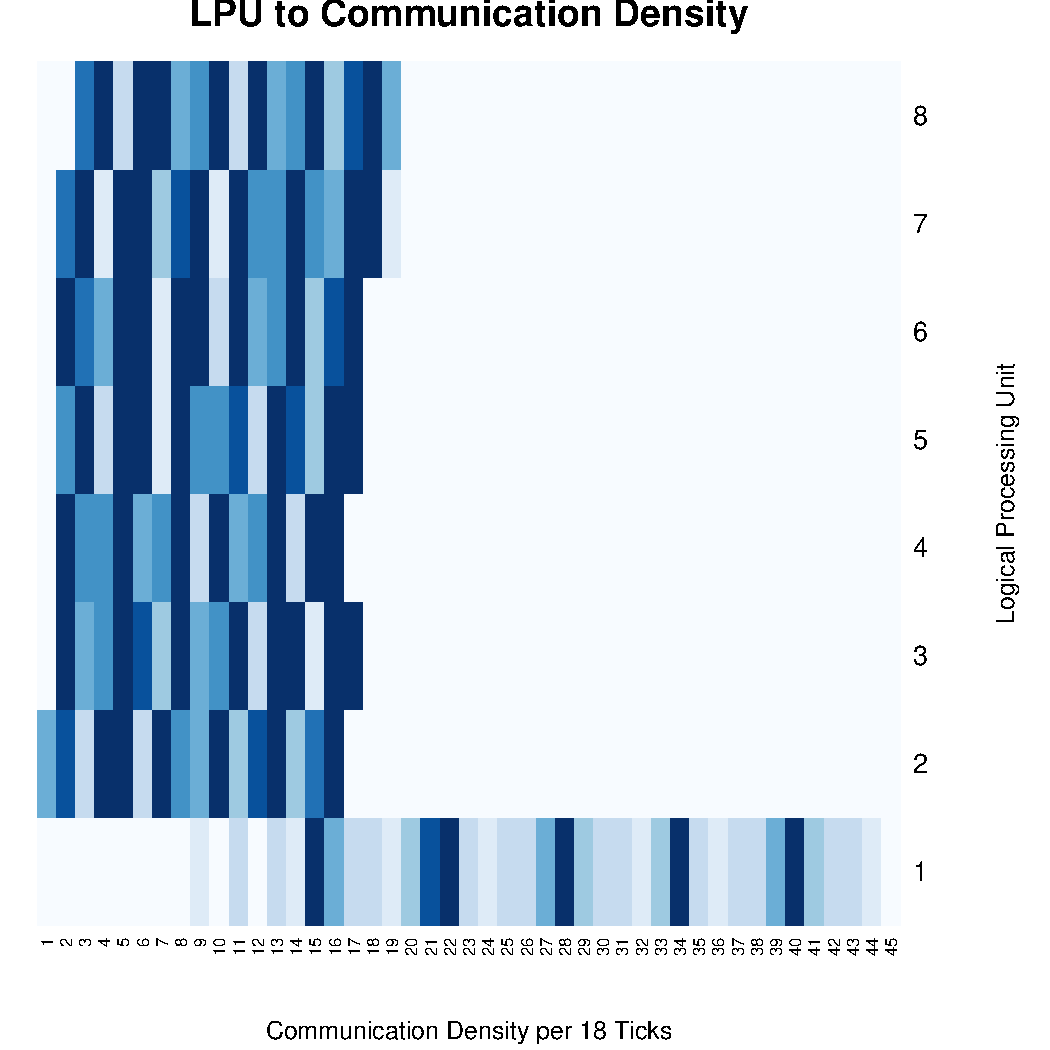
\includegraphics[scale=0.35]{pring-erlam_sched_multi_ws-commdense.pdf}
\caption{ Example of Communication Density graph for the Work-Stealing scheduler 
on a Core i7 running the $PRing$ (defined in section~\ref{sec:cooperativity testing})
application.}
\label{fig:commdense-example}
%\end{wrapfigure}
\end{figure}

Communication Density for example (see figure~\ref{fig:commdense-example}, 
creates a heatmap based on the frequency of
\emph{yield} events which occur whenever a process attempts a $swap$. Each cell
of the heatmap is a color intensity based on the number of \emph{yield} events 
seen in a given time-slice for a given LPU. This time-slice is where the averages
come into play. R heatmaps have a maximum of $9$ colors, so any range we 
select must be scaled to $9$. However, the constant multiplicand is based on the
mean amount of time $N$ ticks take place across each LPU.
We can obviously tune the accuracy of these averages on a per-LPU basis by
modifying $N$. Anecdotally, this turned out to be advantageous on several 
occasions when debugging scheduler implementations. As decreasing the number of
ticks to average together, increased the number of samples and thus accuracy.

\subsection{Cooperativity Testing}\label{sec:cooperativity testing}

As part of the thought experiment, we needed to implement a decent set of test 
cases which would give us a good coverage of the range of cooperative behaviour
in common applications. 

On one hand we have an axis depicting the amount of parallelism possible in an 
application. A system which is completely parallel, would be one where all 
processes spawned have no dependence on any of the others. For our toolkit, we 
called this behaviour $ChugMachine_N$ (figure~\ref{fig:ChugMachine}) ; where $N$ depicts the number of parallel 
processes. On the other side of the axis, we would have a system which had 
absolutely no parallelism possible. We called this behaviour $PRing_N$ (figure~\ref{fig:PRing}), as it
would spawn $N$ processes in a ring formation and pass a token in one direction.
Each process has a channel to its left and right and would synchronize to the 
right until it receives a token to continue. 

$PRing_N$ also gives an example of full-system cooperation, except we would 
instead like some degree of parallelism possible. To experiment with that, we 
would have to throttle the degree of cooperativity. This behaviour is called
$ClusterComm_{(N,M)}$ (figure~\ref{fig:ClusterComm}) as it spawns $N$ processes and $M$ channels which can be
synchronized with by any process. Note for this system to work with swap 
channels we limit $M$ to be at most $\lfloor N/2 \rfloor$ for all tests. 

$ClusterComm_{(N,M)}$ is also an example of full-system cooperation, we also
want to have a possible case for partial-system cooperation. We begin this range
of experiments with a behaviour which acts like a bunch of $ClusterComm_{(N,1)}$
running in parallel. We call this special case behaviour $PTree_{(W,N)}$ (figure~\ref{fig:PTree}); where $W$ is 
the number of work groups to run in parallel. This is the cleanest case of 
partial-system cooperation. We would expect to observe obvious clustering of 
processes by work-group affiliation if the scheduler was 
cooperativity-conscious.

However, to expand on the concept of partial-system cooperativity, we would 
also like to experiment with lop-sided behaviours where a work-group exists 
along with other processes which may not be affiliated with one another. An 
application like this would be the combination of $ClusterComm_{(N,M)}$, 
$ChugMachine_N$, and/or $PRing_N$ running in parallel. For this reason, we made
our behaviours composable.

We are missing two important behaviour simulations: application phase changes,
and hanging processes (typical of I/O bound processes). In the case of the 
latter, a simple built-in command $hang$ was provided which would simulate 
hanging for a random amount of time before allowing the process to proceed with
evaluation. If a scheduler attempted to reduce the process before the $hang$ 
time was completed, it would be immediately preempted. The behaviour which 
implements this is called $UserInput_{(T,C)}$ (figure~\ref{fig:UserInput}); where $T$ is the max time in seconds
the process would hang before continuing, and $C$ is the number of times it 
would simulate ``waiting for user input''. This simple behaviour would also
compose with the others.

For the former missing behaviour, phase changes, we decided to make a variation
of $PTree_{(W,N)}$ called $JumpShip_{(W,P)}$ (figure~\ref{fig:JumpShip}) which would act like $PTree_{(W,N)}$ but would
``change phase'' $P$ times before completion. The act of ``changing phase'' would 
be the successive relocation of all the processes from one work-group to 
another, effectively having all processes from work-group $X$ ``jump-ship'' to
$X+1$ \textbf{mod} $N$.

We would have liked to possibly experiment with variations on the ``jump-ship''
behaviour so as to inject phase changes into $PRing_N$ (by perhaps reversing
direction) or $ClusterComm_{(N,M)}$ (by switching to $ChugMachine_N$ for a 
brief period before returning to $ClusterComm_{(N,M)}$). Yet time constraints
have limited us to the aforementioned.

\begin{figure}
\subfigure[t][Graphical representation of $PTree$, $N$ Parallel work groups.]{
    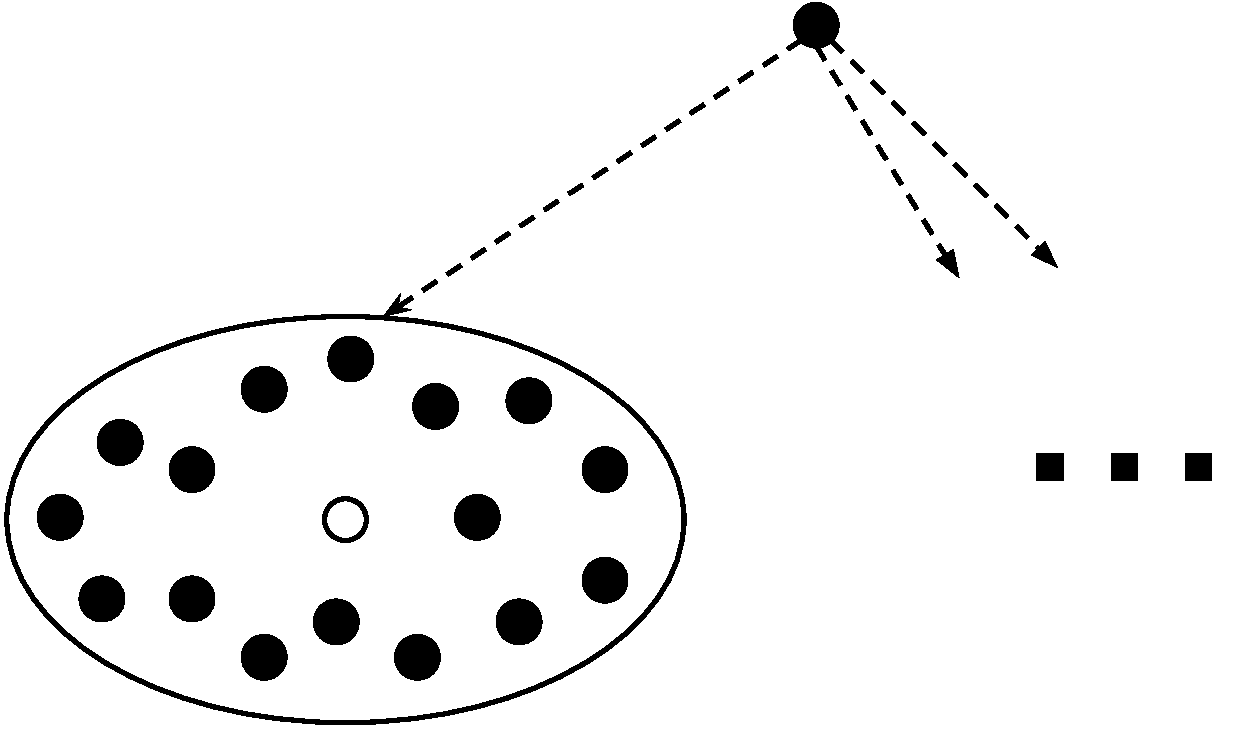
\includegraphics[scale=0.35]{PTree.pdf}
    \label{fig:PTree}
} 
\hfill
\subfigure[t][Graphical representation of $PRing$, full system predictable cooperation.]{
    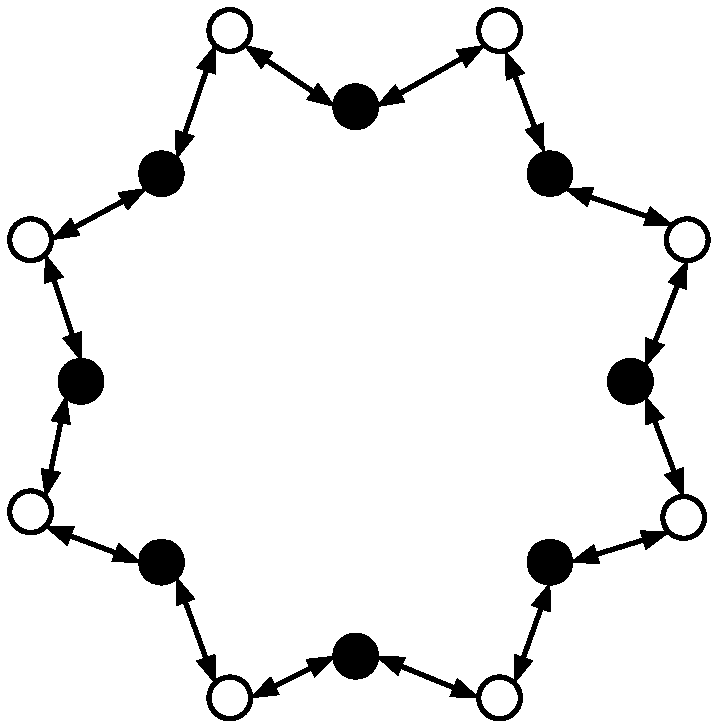
\includegraphics[scale=0.35]{PRing.pdf}
    \label{fig:PRing}
}

\subfigure[t][Graphical representation of $ClusterComm$, $N$ processes to $M$ channels for unpredictable full system cooperation.]{
    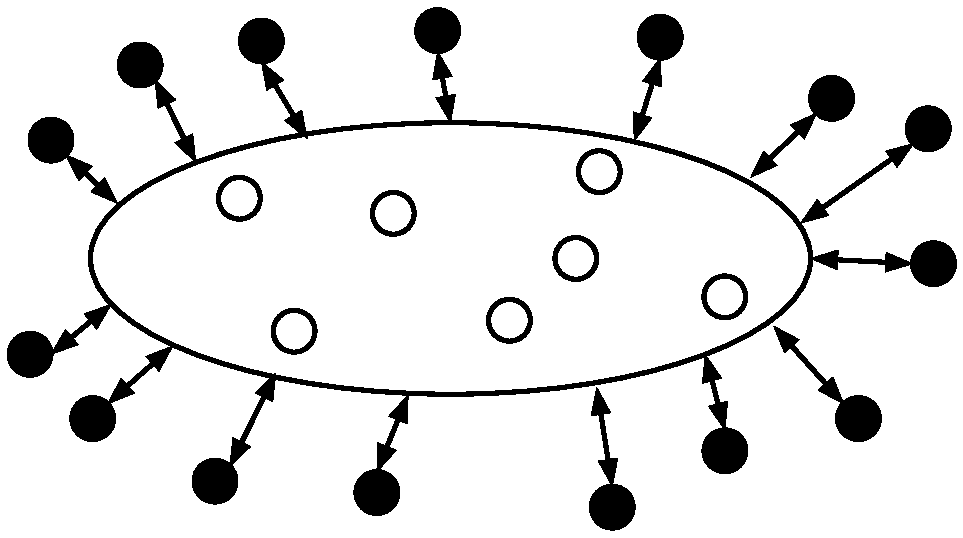
\includegraphics[scale=0.35]{ClusterComm.pdf}
    \label{fig:ClusterComm}
}
\hfill
\subfigure[t][Graphical representation of $ChugMachine$, $N$ worker processes without cooperation.]{
    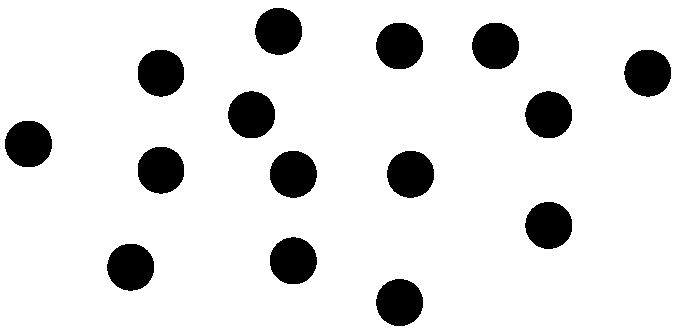
\includegraphics[scale=0.45]{ChugMachine.pdf}
    \label{fig:ChugMachine}
}

\subfigure[t][Graphical representation of $UserInput$, single randomly hanging process.]{
    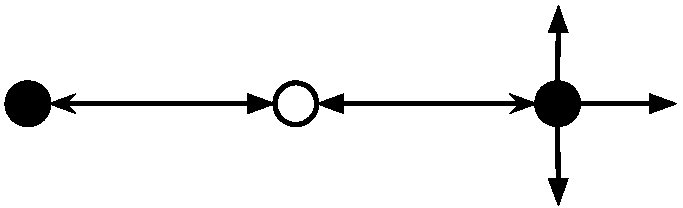
\includegraphics[scale=0.55]{UserInput.pdf}
    \label{fig:UserInput}
}
\hfill
\subfigure[t][Graphical representation of $JumpShip$, $N$ Parallel phase shifting work groups.]{
    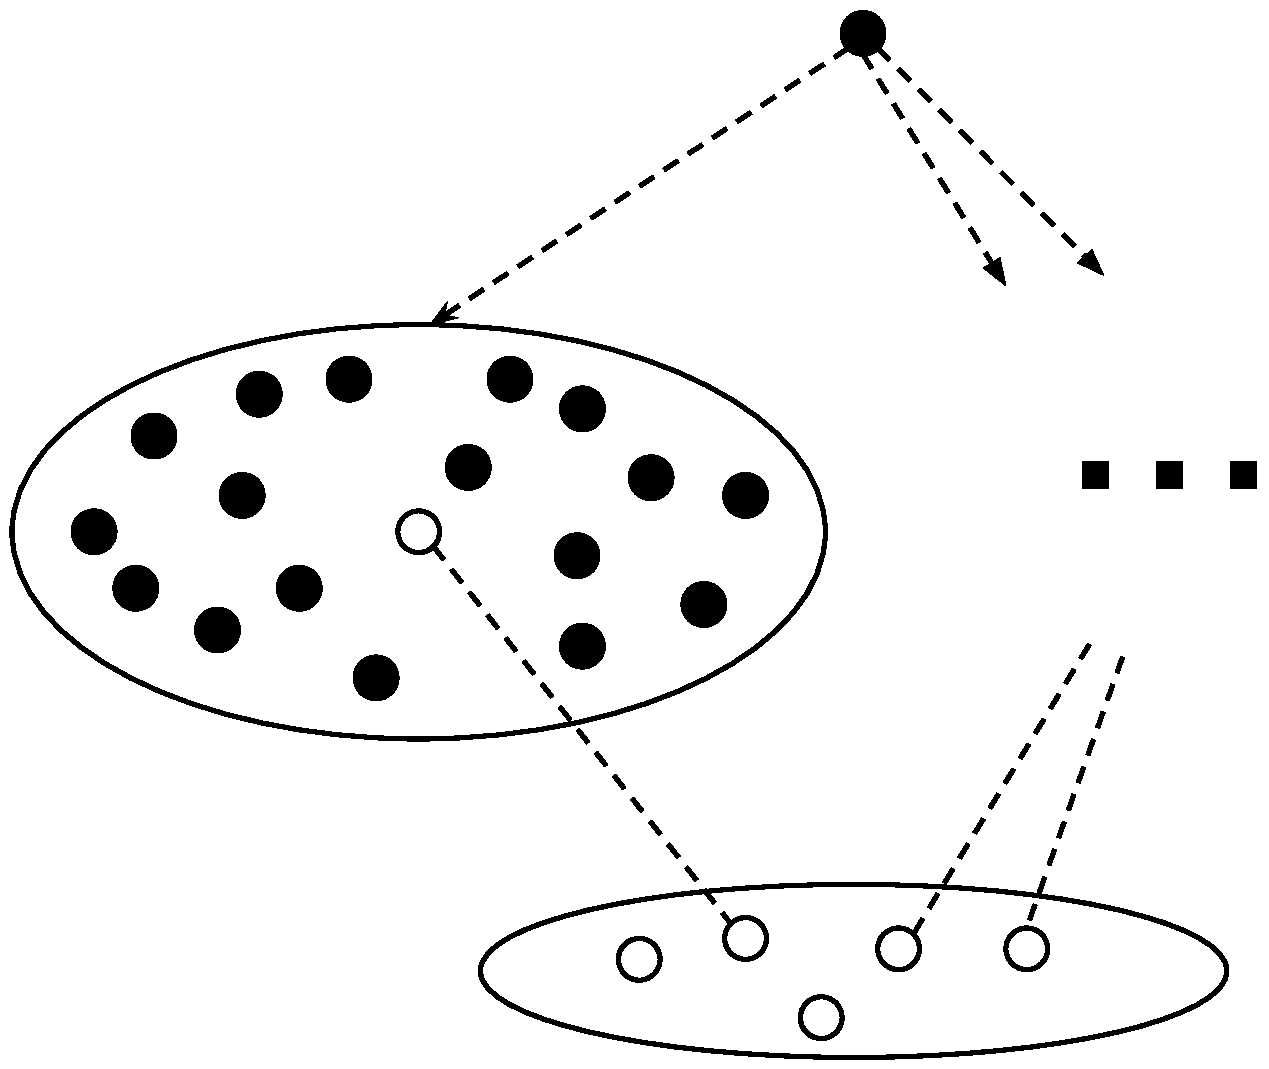
\includegraphics[scale=0.35]{JumpShip.pdf}
    \label{fig:JumpShip}
}
\caption{Simulated behaviour examples and test primitives.}
\end{figure}


\section{Cooperativity Mechanics}\label{sec:cooperativity mechanics}

As mentioned previously, ErLam provides a number of feedback-enabled 
cooperativity-conscious schedulers for comparison purposes. Through our 
exploration of cooperative behaviour we noticed that
cooperativity has, on some level, been captured in previous scheduling systems.
Through techniques keeping in mind cache locality, channel efficiency,
and work-stealing efficiency, we see a common theme of keeping processes which
communicate together, in close proximity. 

Ultimately cooperativity gives us a mechanism for recognizing when processes 
may be moving along the spectrum of application parallelism. We would therefore 
like to look at systems which recognise particular behaviours which utilize this.

\subsection{Longevity-Based Batching}\label{sec:longevity based batching}

As we've mentioned before, batching processes together has been a common 
mechanism in capturing some of the lost efficiency of cache locality. To take
advantage of the cache a message passing language is required to be considerate 
of their channel implementation to allow for it. For example, occam-$\pi$ makes sure
their channel fits into a single 32 bit cache line (technically two, as they
have asymmetrical channels and split it based on send and receive).

However, ErLam elevates the concerns of cache locality into an issue of process 
locality by relying only on symmetrical message passing. Note that 
a channel is loaded into memory at the location (\ie~LPU) of whichever process 
first blocks it and then again at whichever process unblocks it. Thus to reduce
the number of times the channel needs to be loaded, we can still use the 
batching mechanism. Namely, if two processes are communicating frequently, the
channel never needs to be migrated if they exist in the same batch and thus on the
same LPU. This mechanism would be applicable to any other language which uses 
message passing too.

However, this batching mechanism is great when the application is going through
a phase of frequent communication and thus fine-grained parallelism. But in the
event the phase changes or the system is coarse-grained, then a batch actually
harms the ability of the scheduler to parallelize to the fullest. This issue 
however is one we've seen before, the struggle of computation and communication
bound processes.

The CML Interactivity based scheduler breaks up the processes into groups of
long running (computation-bound) and short running (communication-bound)
processes. We can take advantage of this in our case by kicking processes which
are too long-running out of a batch (into a singleton batch for example). To 
merge communicating processes back together in the same batch would be as easy
as turning on Process Absorption for our channels. A process would then be
batched with processes that have all begun communicating on a particular set
of channels.

The mechanism we just described has been implemented as the Longevity-Based
Batching Scheduler. A process belongs to a batch as long as it does not exceed
its quantum (reduction count). If it is preempted, it is thusly kicked out 
from the batch it's a part of (unless it's a singleton). There are of course
alternatives to this (\eg~allow for $N$ quantum to pass before kicking a 
process from a batch), but we, for testing purposes, can just extend the size
of the quantum for the same effect.

To gain entry back into a batch, all a process needs to do is perform a swap 
with Process Absorption turned on. Note as Process Absorption must be toggled
on for this to work, we can experiment with max-parallelism possible in the 
application. Our assumption prior to experimentation was that, the 
longevity-batching scheduler would drop-down into a common work-stealing
scheduler in the worst case (\ie~all processes are singleton batches). We talk 
more on these assumptions and their validity in Chapter~\ref{chap:results}.


\subsection{Channel Pinning}\label{sec:channel pinning}

An alternative approach to batching, which moves the channels to the processes,
is to set an affinity to a core based on which channels you cooperate on. We 
call this mechanism Channel Pinning, as we bind a channel upon creation to a
particular LPU and force processes to that location to perform a swap. 
There are a large number of interesting mechanics for this behaviour. But we 
will look at three: 
\begin{inparaenum}
\item How to spread the channel pinnings?
\item How should processes react when attempting a swap on a remotely bound channel?
\item And based on the decisions made in the previous, how should a scheduler steal/spawn a process?
\end{inparaenum}

When choosing a channel spread algorithm there are two things which need to be
compared, cost of creating a channel and channel usage of the running application. 
In stark contrast to the previous scheduler, channel
pinning would either need to be an expensive heuristic or a programmer-aided
decision based on the application itself.
For example, if our channel pinning algorithm was a sane even spread across all
processors we would have ignored the possibility that a subset of the channels
could be used more frequently. This could therefore cause more harm than good.
If we chose to do an expensive check across all processors to compute the 
saturation each time we create a channel we would be harming the application 
which uses a map-reduce style, and uses a lot of temporary one-use channels.

On top of this complication, this also ignores the possibility of phase changes.
It may be the case that during a start up phase, the frequency of particular 
channel usage may offset the saturation to such a degree that any further 
checks will suggest alternate processors despite possibly being inaccurate.
However, these issues are beyond the scope of this discussion and we will 
instead focus on scheduling around channel pinning. As such we only provide the
following channel pinning implementations: 
\begin{inparaenum}
\item \emph{same}, which pins the channel to the same processor it is created 
    on (\ie~ the processor which evaluates $newchan$).
\item \emph{even}, which pins the channel in a round-robin fashion starting at
    LPU $0$.
\end{inparaenum}

Note \emph{same} pinning, would not be ideal for an application which creates
all channels in one process and then hands them out to its children like in
$JumpShip_{(W,P)}$, or $ClusterComm_{(N,M)}$. However, \emph{even} pinning will
be perfect for them. We expect experimentation with composed application will
have interesting effects in this scheduler.

We have a couple of possible mechanisms for how a process should be handled when
it comes time to communicate. In the event it is wanting to communicate on a 
channel that is not local, we propose the following mechanism: let them anyway
but if they block, spawn them to the LPU which owns the channel.

The theory for this is, in the event of a block, the local LPU won't gain 
anything from having it in its queue (if process absorption is turned on it would 
loose it anyway). However, if the process completes a swap, both the remote
LPU and the local can continue in parallel.

Due to this selective spawn feature, we have the opportunity to look at a 
selective steal opportunity. Namely, when stealing we can attempt to grab from
a random scheduler, one or more processes which have communicated with a 
randomly selected channel which the thief owns. This is akin to the children's
card game "Go Fish" where in our case a scheduler may ask if another "has any
channel 3's".

However, with this mechanism it may be the case that there is never any work
for a particular scheduler. In this case, we have added the post condition that
if a process has never communicated, or if the scheduler is not the owner of a
channel, then they act as wild cards and can match anything. This is both a 
simplistic algorithm, but it also makes sure the scheduler falls back to a 
standard work-stealing algorithm by default.

We now note that the primary interest in comparing this scheduler is to look at 
this work-stealing mechanism.
We would like to see how this type of mechanism fairs against both a best and
worst case scenario. We first thought the worst case scenario would be a 
$ChugMachine_N$ due to the reliance on wild-cards, however after more 
consideration a single $ClusterComm_{N,1}$ may end up having a worse behaviour
due to the constant re-spawning of processes back to the owner of the primary
channel. A best case in this scenario would be a $PTree_{(W,N)}$ when $W$ is greater than or equal
to the number of processing units available.

\subsection{Bipartite Graph Aided Sorting}
    \label{sec:bipartite graph aided sorting}

Both of the previous schedulers ignore the effects ordering
can have on execution behaviour. We hypothesize that order of process execution
could have a drastic consequence on highly cooperative processes by pairing 
channels such that if a process where to block, the unblock would happen as soon
as possible (\ie~the scheduler would not choose a process which had no probability of unblocking it).

Granted the extreme of this type of scheduler would be excruciatingly unfair, and
as such we still maintain a round-robin like behaviour, except now we rely on 
a sorted process queue. Sorting the process queue would allow us the chance to 
increase the likelihood of immediately unblocking a blocked channel, while still
maintaining execution fairness. 
Sorting the process queue would also have the aided side effect of making 
work-stealing potentially more efficient when stealing more than one from a 
victim queue. Namely, it would be much more likely that the group of processes
stolen are cooperating. 

Due to this, we hope to show an interesting case where process absorption may 
not be the preferred channel implementation. The blocking channel, one which will
immediately return, will allow for the process to stay sorted and allow for the 
next process following it to unblock it for its next turn. Thus relying on 
work-stealing alone to migrate processes in a potentially smarter and 
more-grouped way.

There are three metrics which could effect the order of processes, and which would
subsequently trigger a resorting of the process queue. A process yielding, 
returning, or spawned could all mean that a particular process or set of 
processes should to be relocated. However, frequent sorting may cause the scheduler's
fairness to suffer. We therefore set a variable, $\Gamma$ which defines how many 
"events" can happen before causing a resort.

To provide a mechanism for sorting, we structure our process queue as a bipartite 
graph, where one side is our process queue, and the other is the set of channels.
We generate a ``pseudo-priority'' based on recency of the communications over
the number of channels it has communicated with. Namely, we sort the process queue
by $\Delta(P_i) = \Sigma E_i / |C_i|$ where $E_i$ is the edge set of timestamps,
and $C_i$ is the set of channels $P_i$ communicated with. The default priority function, $\Delta$,
is intended to give our processes which communicate frequently, a head start, and
all other processes can be pushed to the end (and more likely stolen). 

If our process queue is long, we maintain preferential treatment for the set of 
interactive processes. If our process queue is short, then the effects of 
sorting are negligible. As such, we should only be concerned with sorting 
a process queue after a particular size. This is another chance for heuristic
analysis. Due to this though, we would expect to see poorer behaviour on most
simple simulated applications, but would steadily gain in advantage when 
subjected to composed applications.

